\documentclass[10pt,twocolumn,letterpaper]{article}

\usepackage{cvpr}
\usepackage{times}
\usepackage{epsfig}
\usepackage{graphicx}
\usepackage{amsmath}
\usepackage{amssymb}

% Include other packages here, before hyperref.

% If you comment hyperref and then uncomment it, you should delete
% egpaper.aux before re-running latex.  (Or just hit 'q' on the first latex
% run, let it finish, and you should be clear).
\usepackage[breaklinks=true,bookmarks=false]{hyperref}

\cvprfinalcopy % *** Uncomment this line for the final submission

\def\cvprPaperID{****} % *** Enter the CVPR Paper ID here
\def\httilde{\mbox{\tt\raisebox{-.5ex}{\symbol{126}}}}

% Pages are numbered in submission mode, and unnumbered in camera-ready
%\ifcvprfinal\pagestyle{empty}\fi
\setcounter{page}{4321}
\begin{document}

%%%%%%%%% TITLE
\title{Visualizing sub-networks in deep convolutional neural networks}

\author{First Author\\
Institution1\\
Institution1 address\\
{\tt\small firstauthor@i1.org}
% For a paper whose authors are all at the same institution,
% omit the following lines up until the closing ``}''.
% Additional authors and addresses can be added with ``\and'',
% just like the second author.
% To save space, use either the email address or home page, not both
\and
Second Author\\
Institution2\\
First line of institution2 address\\
{\tt\small secondauthor@i2.org}
}

\maketitle
%\thispagestyle{empty}

%%%%%%%%% ABSTRACT
\begin{abstract}
   Deep convolutional neural networks have recently demonstrated great success in computer vision problems. While there have been several efforts to understand how how these networks work, we are still far from truth. Moreover, most of the expoloratory work done has been in the domain of understanding object and scene detectors. Our motivation here is two fold - expanding the domain of standard network visualization techniques to the domain of text recognition, and most importantly, suggesting new general purpose visualization pipelines which rely on identifying subnetworks which may be performing a high level function, as opposed to the standard per unit visualization. Such subnetwork identification methods may even be useful in reducing network complexity when invariants of the system are known, and in facilitating transfer learning across different domains of computer vision. 
\end{abstract}

%%%%%%%%% BODY TEXT
\section{Introduction}
Convolutional neural networks have unprecedented success in various computer vision tasks in the recent past.  With applications ranging from object detection \cite{}, segmentation \cite{}, text recognition \cite{}, CNN's have quickly become a staple in the computer vision community. Their success can be partially attributed to the networks ability to learn invariants in the high dimensional space \cite{}. While the idea was first introduced long back by LeCun et al in early 1990s, several factors have controbuted to their unprecedented success - (i) Availability of much larger training sets with millions of labelled samples, (ii) Powerful GPU's and more computational horsepower making it possible to train networks larger than ever, and (iii) better training strategies for regularization using Dropout \cite{wan2013regularization} and batch normalization \cite{ioffe2015batch}.

Despite their successes, CNNs still are not much more than high performing black boxes, with limited understanding about what they have learned, and how they handle different kinds of input. Without a firm understanding of what the CNN is doing, it becomes hard to improve and optimize network typologies and techniques without trial and error. While there are a number of papers working on visualizing the internal representation of hidden layers, most of them have focussed on per-unit visualizations \cite{yosinski2015understanding,mahendran2015understanding,zhou2014object}.Moreover, most of this work has been done in the domain of object/scene detection. We take this one step further by extending these existing techniques to the domain of text recognition, which has seen significant success with CNN's \cite{Jaderberg14,Jaderberg14c,Jaderberg14d}. As text is inherently synthetic data, and because we work with a synthetic dataset, it gives us the power to address aspects which may be missing in object/scene datasets. In particular, transformations such as scaling, rotation, and translation have not been visualized in networks before. 

Further, we believe that keeping in sync with the idea that a network involves computations chained together it makes more sense to visualize a chain of operations as opposed to a single node. To address this, our work attempts to  explore different visualization techniques which aim to identify a sub-network, or a path of information flow in the network which may be related closely with either (i) A particular kind of input image, or (ii) A particular kind of output class. We propose a method akin to how a neurologist would use functional magnetic resonance imaging to map out the brain by mapping out regions of activity while performing specific tasks.\cite{friston1998event} We experimentally demonstrate the our visualization techniques for transformations by using a network trained to read text in the wild. 

Identifying sub-networks can prove to be extremely useful at different steps in CNN training and deployment. It can help decide leaner network architecture depending upon known invariants in the training dataset, and prune existing networks without reducing accuracy over certain datasets. Furthermore, it can, in principle, facilitate a plug-and-play use of sub-networks for transfer learning to new domains akin to the fine-tuning approach which is gaining popularity in the computer vision community. \cite{}

\subsection{Main Contributions}
Our contributions are three-fold:
\begin{enumerate}
\item We Extend standard visualization techniques to a new domain - a state of the art text recognition network.

\item Furthermore, we propose visualization techniques which help identify sub-networks preferentially activated by a certain kind of input images, or instead, lead to the discriminative network predicting a certain output class. This extends the existing capabilities of network visualization techniques from per-unit analysis to analyzing a meaningful chunk of nodes at a time. 
\item \color{red} Finally, we explore the benefits that sub-network identification makes possible, including a demonstration of detecting an removing transformation specific units in a network.
\end{enumerate}

\subsection{Main Limitations}
Our visualization technique can be useful for visualizing the network if the units of interest exist in the convolutional layers. If instead they exist in the fully connected layers, not much useful information can be extracted. In addition it is difficult to apply isolated pruning without effecting the entire network.

Another limitation is that pruning the networks graphs may not have a computational boost on hardware that are designed to work with large amount of vectors in parallel, such as GPUs. However, as machine learning becomes more prevalent, applications that utilize lower powered simpler devices will increase and benefit from the computation reduction.

\section{Related Work}
\subsection{CNN Visualization}
With the advent of CNN's, has been a growing interest in the both the computer vision and the deep learning community to understand the functionings of these models. Most recent works build on creating natural pre-images \cite{DBLP:journals/corr/MahendranV15} that maximally activate certain nodes of the network, or obtaining saliency maps from these networks using techniques like deconvolution \cite{DBLP:journals/corr/ZeilerF13} and
projecting back fully connected layers. \cite{DBLP:journals/corr/SimonyanVZ13}. However, most work in this field has been limited to the domain of object and scene detectors, and use a single neuron as the basis of the visualization, identifying exemplar neurons that strongly correspond to high level features.\cite{zhou2014object,DBLP:journals/corr/GirshickDDM13,DBLP:journals/corr/MahendranV15,DBLP:journals/corr/ZeilerF13,DBLP:journals/corr/SimonyanVZ13,mahendran2015understanding}. Our work extends adaptations of many of these standard techniques \cite{yosinski2015understanding} to the domain of text recognition. Furthermore, we have proposed two new techniques that take a more zoomed out perspective to network visualization by studying the activations of several units at the same time. 

\subsection{Text Recognition}

The computer vision community has been working on the problem of recognizing text in natural scenes for long a time now\cite{1315187}. While varied approaches have been tried to these problems, the standard approach has been to split the problem in two parts - text detection and text recognition \cite {}. The advent of deep learning has led to state of the art papers utilizing the power of CNN's. \cite{}



\section{Datasets and Model}
\subsection{DATASETS}
Talk about MJSynth and Synthetic dataset we generated. 

\subsection{Synthetic text generation pipeline} \label{sec:synthtext}
Specialized datasets were necessary for the subnetwork identification visualization technique described in section \ref{sec:subnetwork}.
To generate these datasets a modified version of SynthText \cite{Gupta16} was used. This allowed us to quickly create test examples with specified constraints. The constraints experimented with included \textcolor{red}{text color, rotation, width, and border}. We generated \textcolor{red}{~1000} test examples for each constrained parameter. Examples of generated text are shown in Fig. \ref{fig:genText}.

\begin{figure}
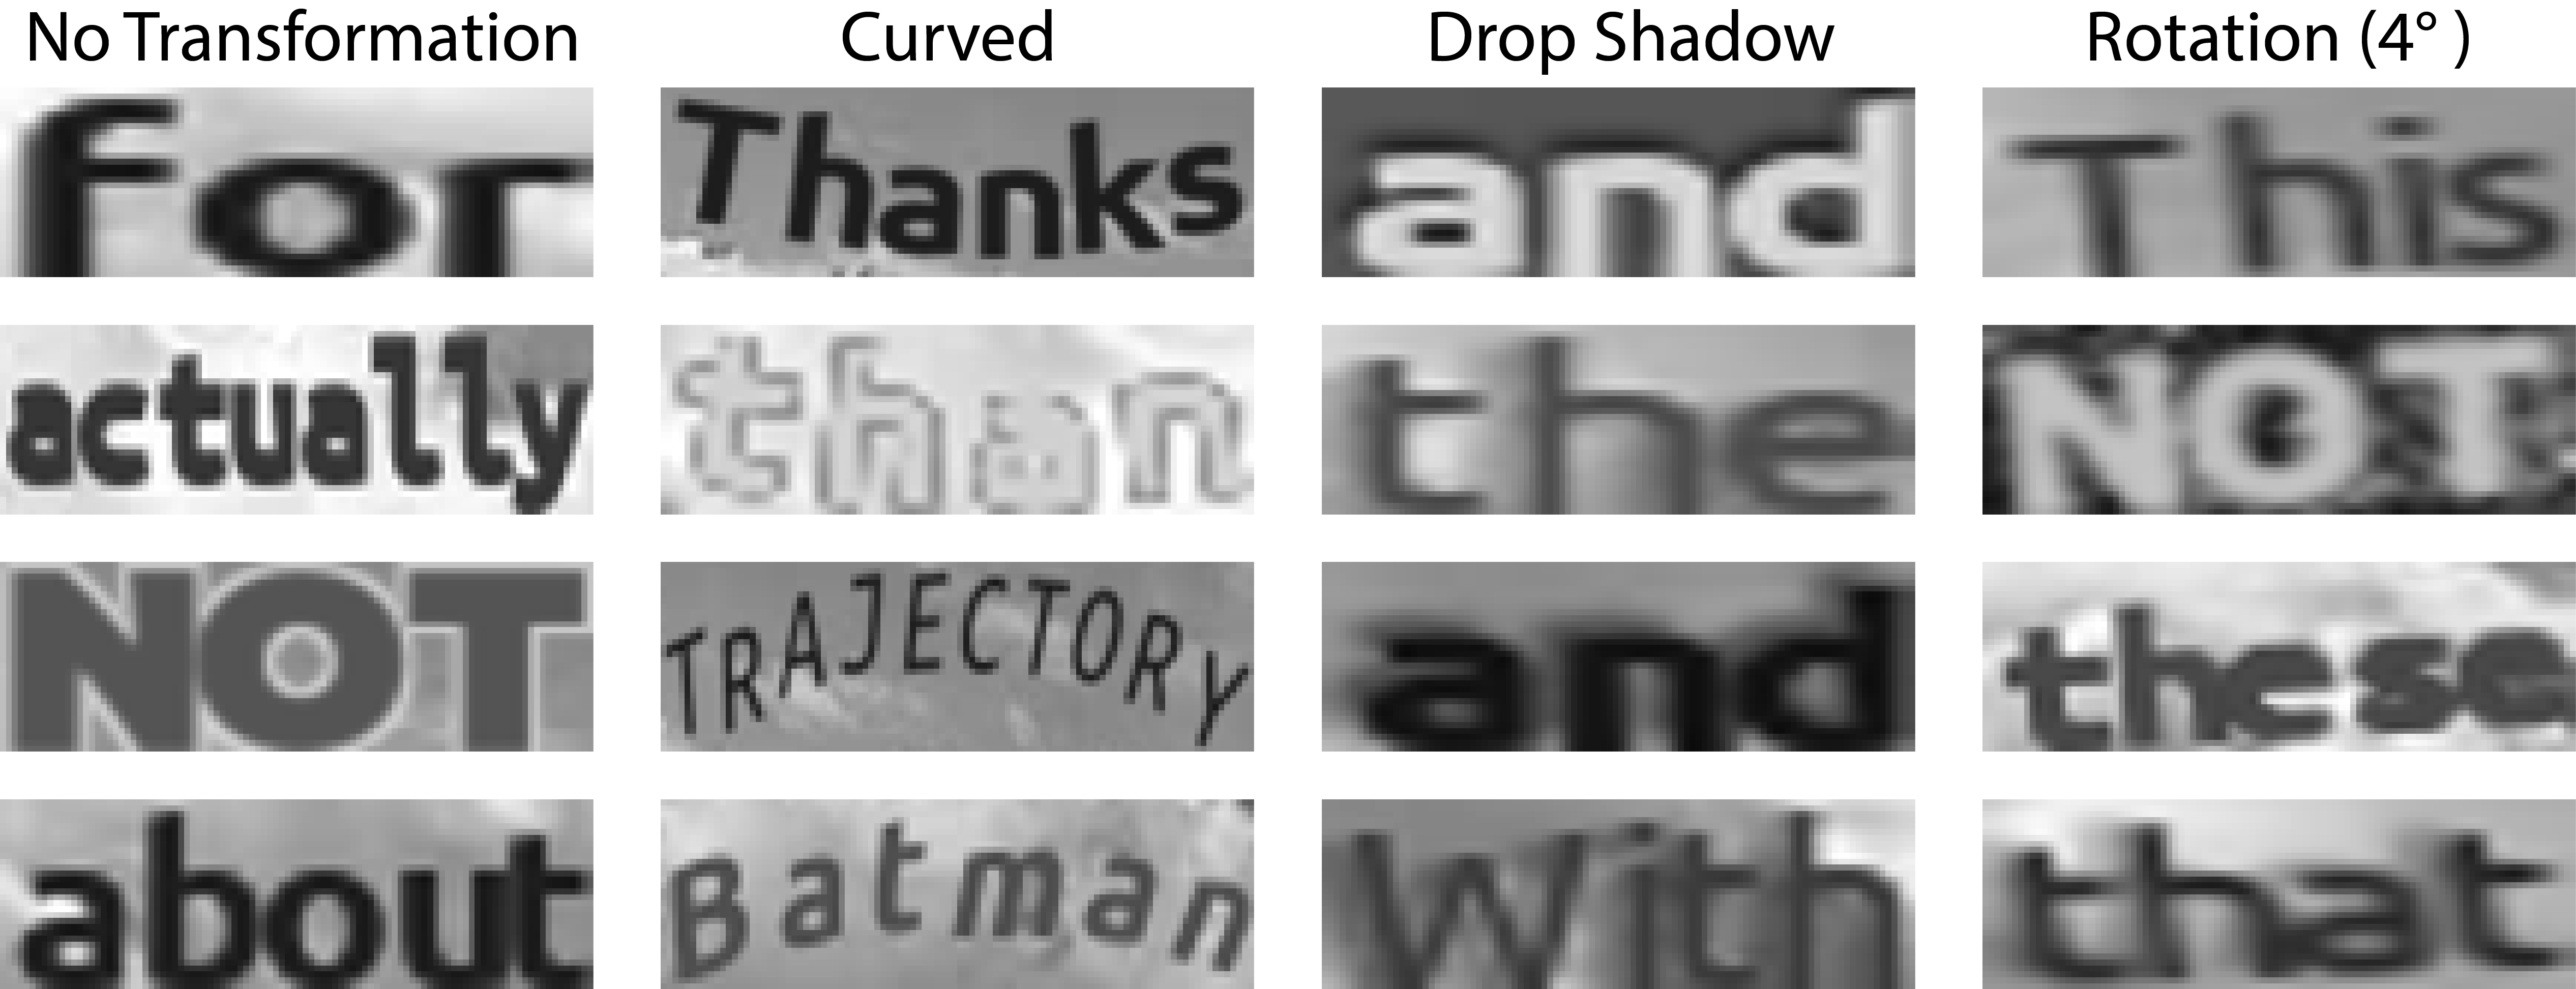
\includegraphics[width=\columnwidth]{Figures/synthtext_outputs/synthext_outputs.png}
\caption{Example of generated text from a sample of four different text constraints. The ability to create large test sets with different constraints allows us to compare differences in network activations.}
\label{fig:genText}
\end{figure}

\subsection{NIPS15 model}
Describe charnet and oxford pipeline

\subsection{Model Validation}
Give numbers on model validation for MatConvnet and Caffe implementation.

\subsection{Dropping Neurons}
How we choose what and when to drop neurons

\section{Visualization Pipelines}

\subsection{Deep Visualization Toolbox by yosinski et al}

\subsection{Visualizing filter activations}

\subsection{Network architecture invariants - Top Activations Method}

\subsection{Location encoding in networks - Patch Method}

\subsection{Activation Signature through difference maps} \label{sec:subnetwork}
We propose a method to isolate subnetworks by using activations. Similar to how a neurologist would map the brain, we probe the network with different datasets and observe how the network reacts. Our method focuses on the amount of activation at each node. As an example assume we are interested in finding a subnetwork associacted with specific transformation. First two specialized synthetic datasets are generated as described in section \ref{sec:synthtext}. In this case one dataset does not have the transformation and the other does. The datasets are fed through the network and the activations are recorded and visualized. To visualize the activations, each filter output is \textcolor{red}{averaged}. Each of these resulting values are \textcolor{red}{averaged} over all of the test inputs. Finally the resulting values are mapped on a 2d plane as shown in Fig. \ref{fig:subvis}. \textcolor{red}{In practice we found that visualizing after RELU operations was beneficial as the dropped negative values provided little value.} Two maps are created, $V_0$ and $V_1$, for the dataset with and without the transformations. Comparisons between $V_0$ and $V_1$ can be used to get and idea of how the network reacts differently. With experimentation we found the following metric the most valuable for visualizations: \textcolor{red}{$$\frac{|V_0-V_1|}{V_0}$$}

This method attempts to visualize the structure of the network rather than node specific operations as is typically done. The structure view provides and abstraction that is useful with discussing operations that are difficult or unnecessary to visualize. For example, it is difficult and uninformative to visualize transformations (rotation, scale, translation, etc). However understanding which parts of the network are active during different transformations can be informative.
describer possible uses of this information (here or somewhere else?)||

\begin{figure*}
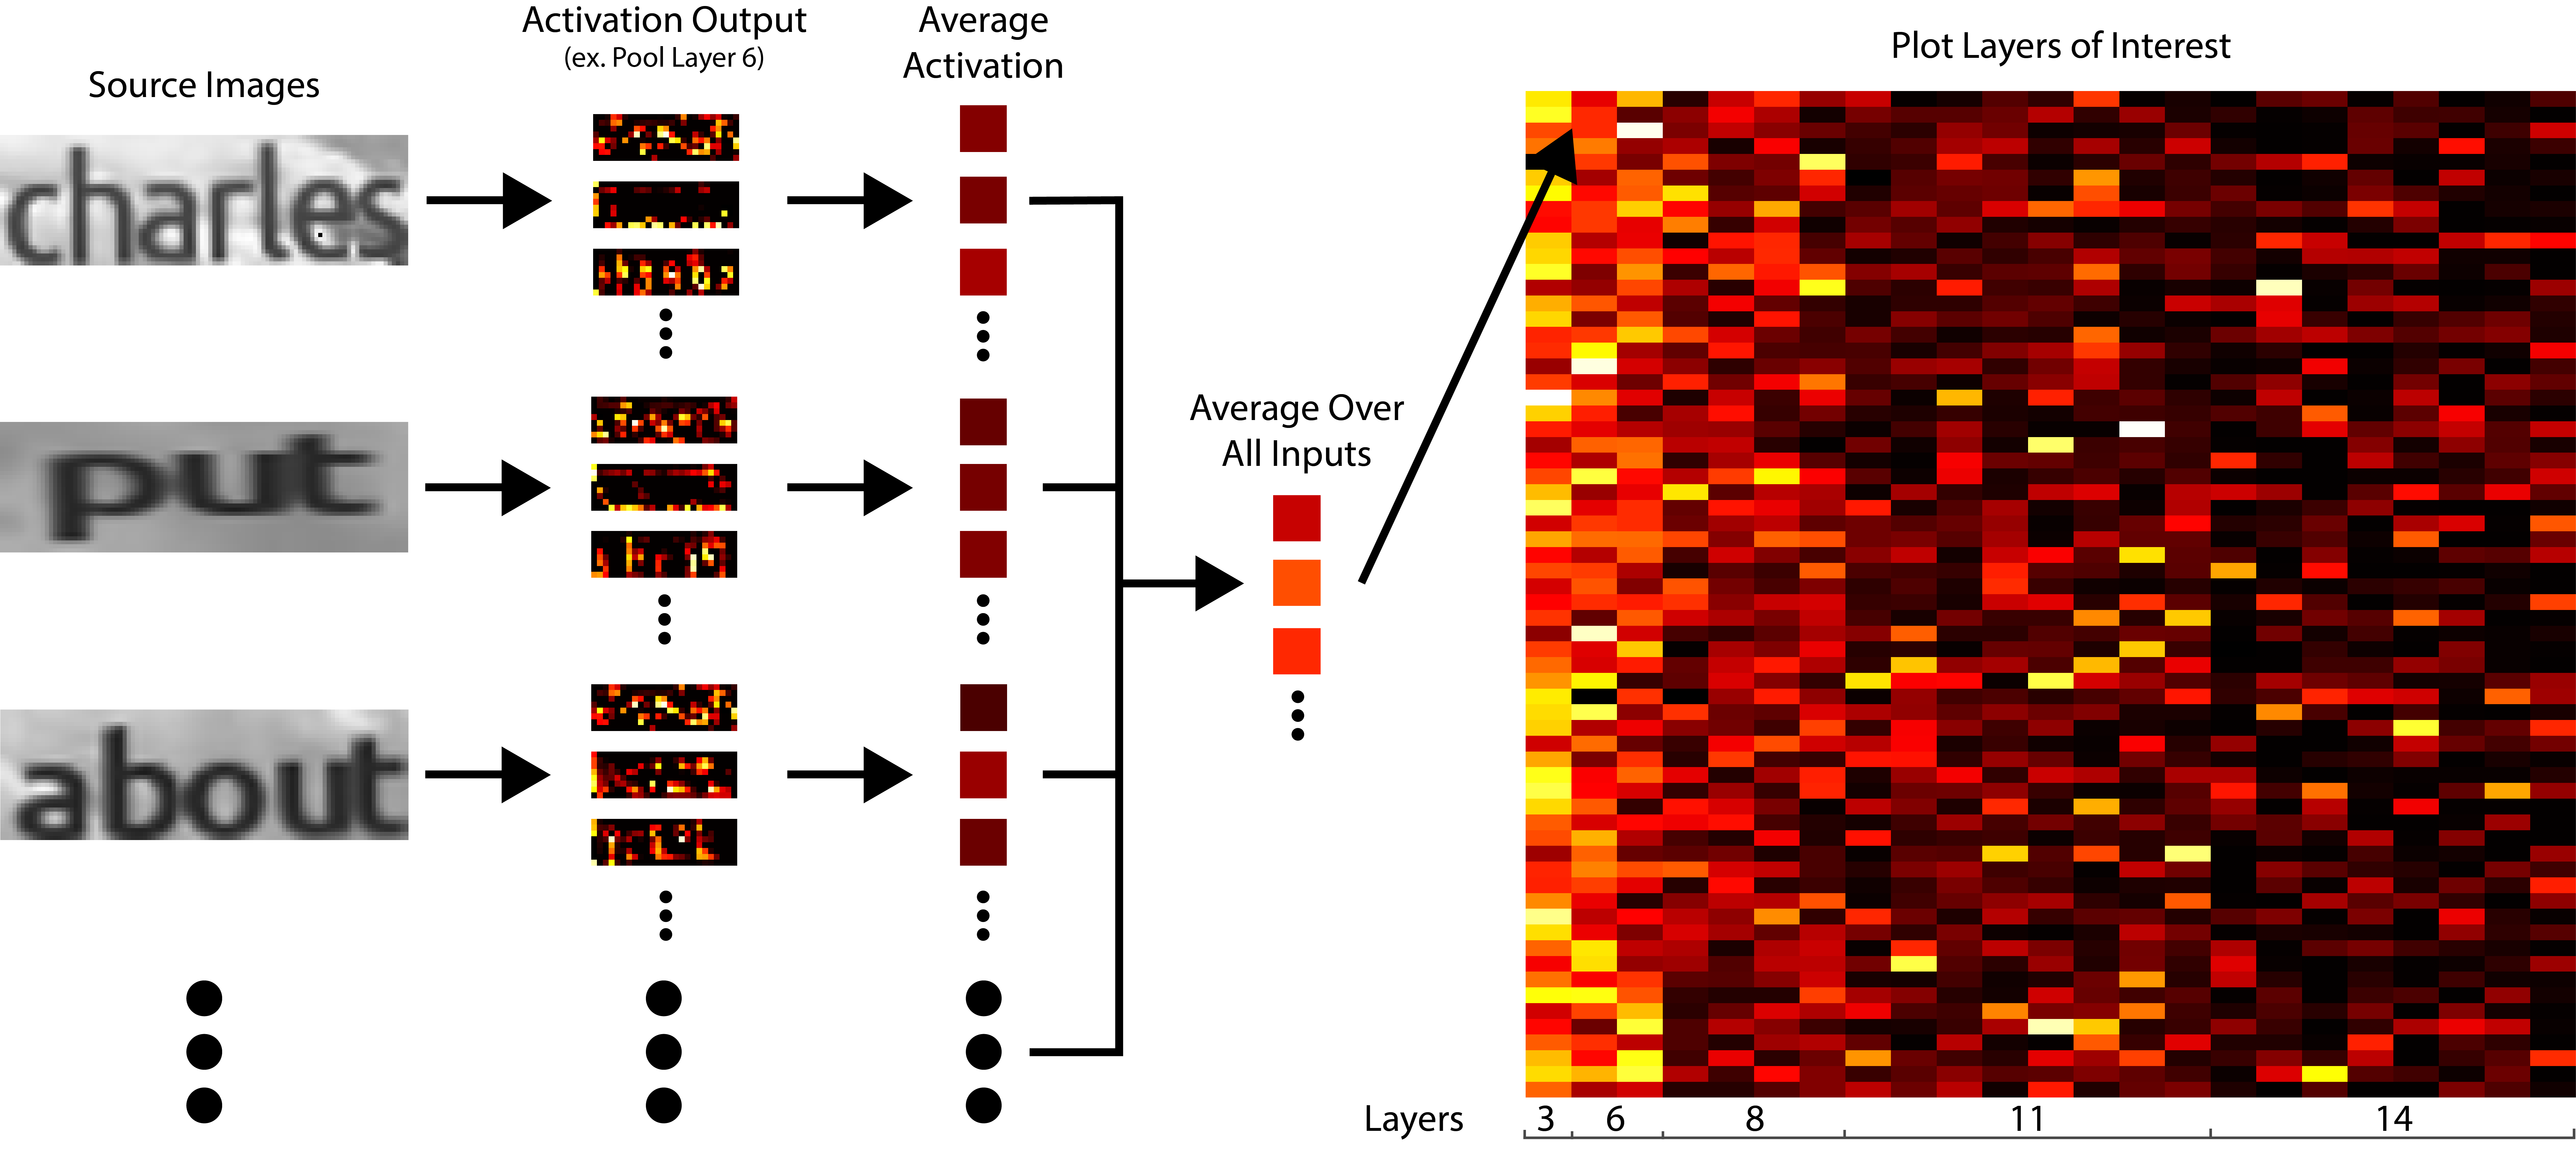
\includegraphics[width=1\textwidth]{Figures/activations_map_overview/act_map_overview-01.png}
\caption{Illustration describing how the activation maps are created. First ~1000 text images are fed through the network. The activation outputs are recorded for each layer. Each individual filter activation is averaged. These averaged activation are then averaged over all of the source images and plotted on a 2D grid. Since the number of filters per layer varies, we give additional columns to layers with more filters (For example layer 8 has 4 columns). This is done to compact the visualization. Information about the choice of layers can be found in the supplement.}
\label{fig:subvis}
\end{figure*}

\section{Results}

\subsection{Detecting Transformation Specific Units}
Show that we can detect transformation units.

\begin{figure}
%\includegraphics[width=\columnwidth]{}
\caption{Comparison of activations for different transformations}
\label{fig:comp}
\end{figure}

\subsection{Dropping Transformation Specific Units}
Show that we retain (or don't) accuracy if we drop units

\begin{figure}
%\includegraphics[width=\columnwidth]{}
\caption{Plot of accuracy decrease as neurons are removed}
\label{fig:comp}
\end{figure}

%-------------------------------------------------------------------------
\section{Discussion}

\subsection{Better understanding of Deep CNNS}
Talk about why this helps us understand what Deep CNNs are doing

%-------------------------------------------------------------------------
\subsection{Transfer Learning}

Talk about how this can better inform transfer learning because we know what is doing what

%-------------------------------------------------------------------------
\subsection{Reducing Computational Complexity}
Talk about why this pruning process may be useful to improve run times on mobile devices (or non GPU devices).

%-------------------------------------------------------------------------
\subsection{Conclusion}
Traditional per-unit visualization tools like the Deepviz toolbox \cite{} show that the text detection network operates similar to an object or scene detector. To get a more zoomed out perspective of the information flow, we proposed two new general purpose techniques for identifying highly activated sub-networks. The Top Activations method attemps to capture the essence of the chained convolutions which make neural networks so successful. The Activation Signature method visualizes the differences in activations corresponding certain input transformations. This helps identify an activation signature for each transformation. These subnetwork identification methods may prove to be useful in debugging and optimizing network architectures as they may help map high level features of the image to regions in the network. Future work includes continuing searching for examplar subnetworks corresponding to particular high level tasks.

%------------------------------------------------------------------------

{\small
\bibliographystyle{ieee}
\bibliography{egbib}
}

\end{document}
